\bframe{Optimal time-dependent modes (OTD)}
\begin{equation*}
  \dot{\mathbf{y}} = \mathbf{K} \mathbf{y}
\end{equation*}

\begin{equation*}
  \dot{\mathbf{Y}} = \mathbf{K} \mathbf{Y} - (\mathbf{Y}^T \mathbf{K} \mathbf{Y}) \mathbf{Y}
\end{equation*}

\eframe

\bframe{Paper}
\begin{center}
  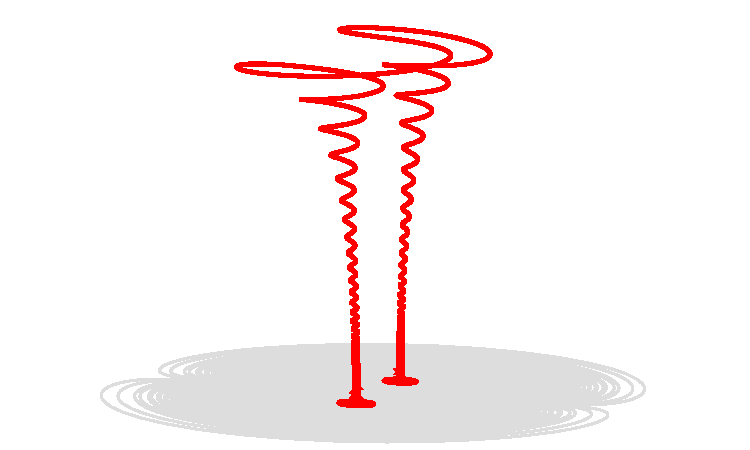
\includegraphics[width=\textwidth]{i/far.pdf}
\end{center}
\eframe

\bframe{Paper}
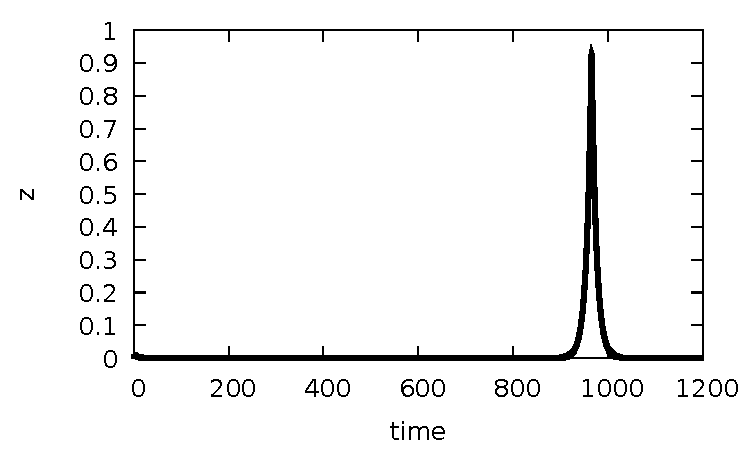
\includegraphics[width=0.5\textwidth]{i/z.pdf}
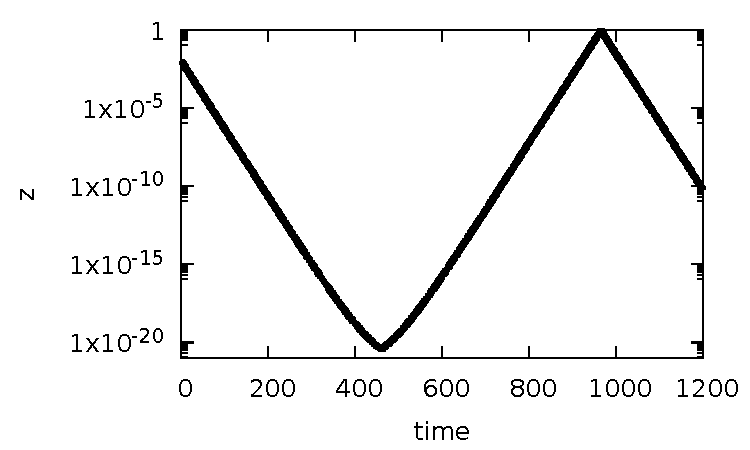
\includegraphics[width=0.5\textwidth]{i/logz.pdf}
\\
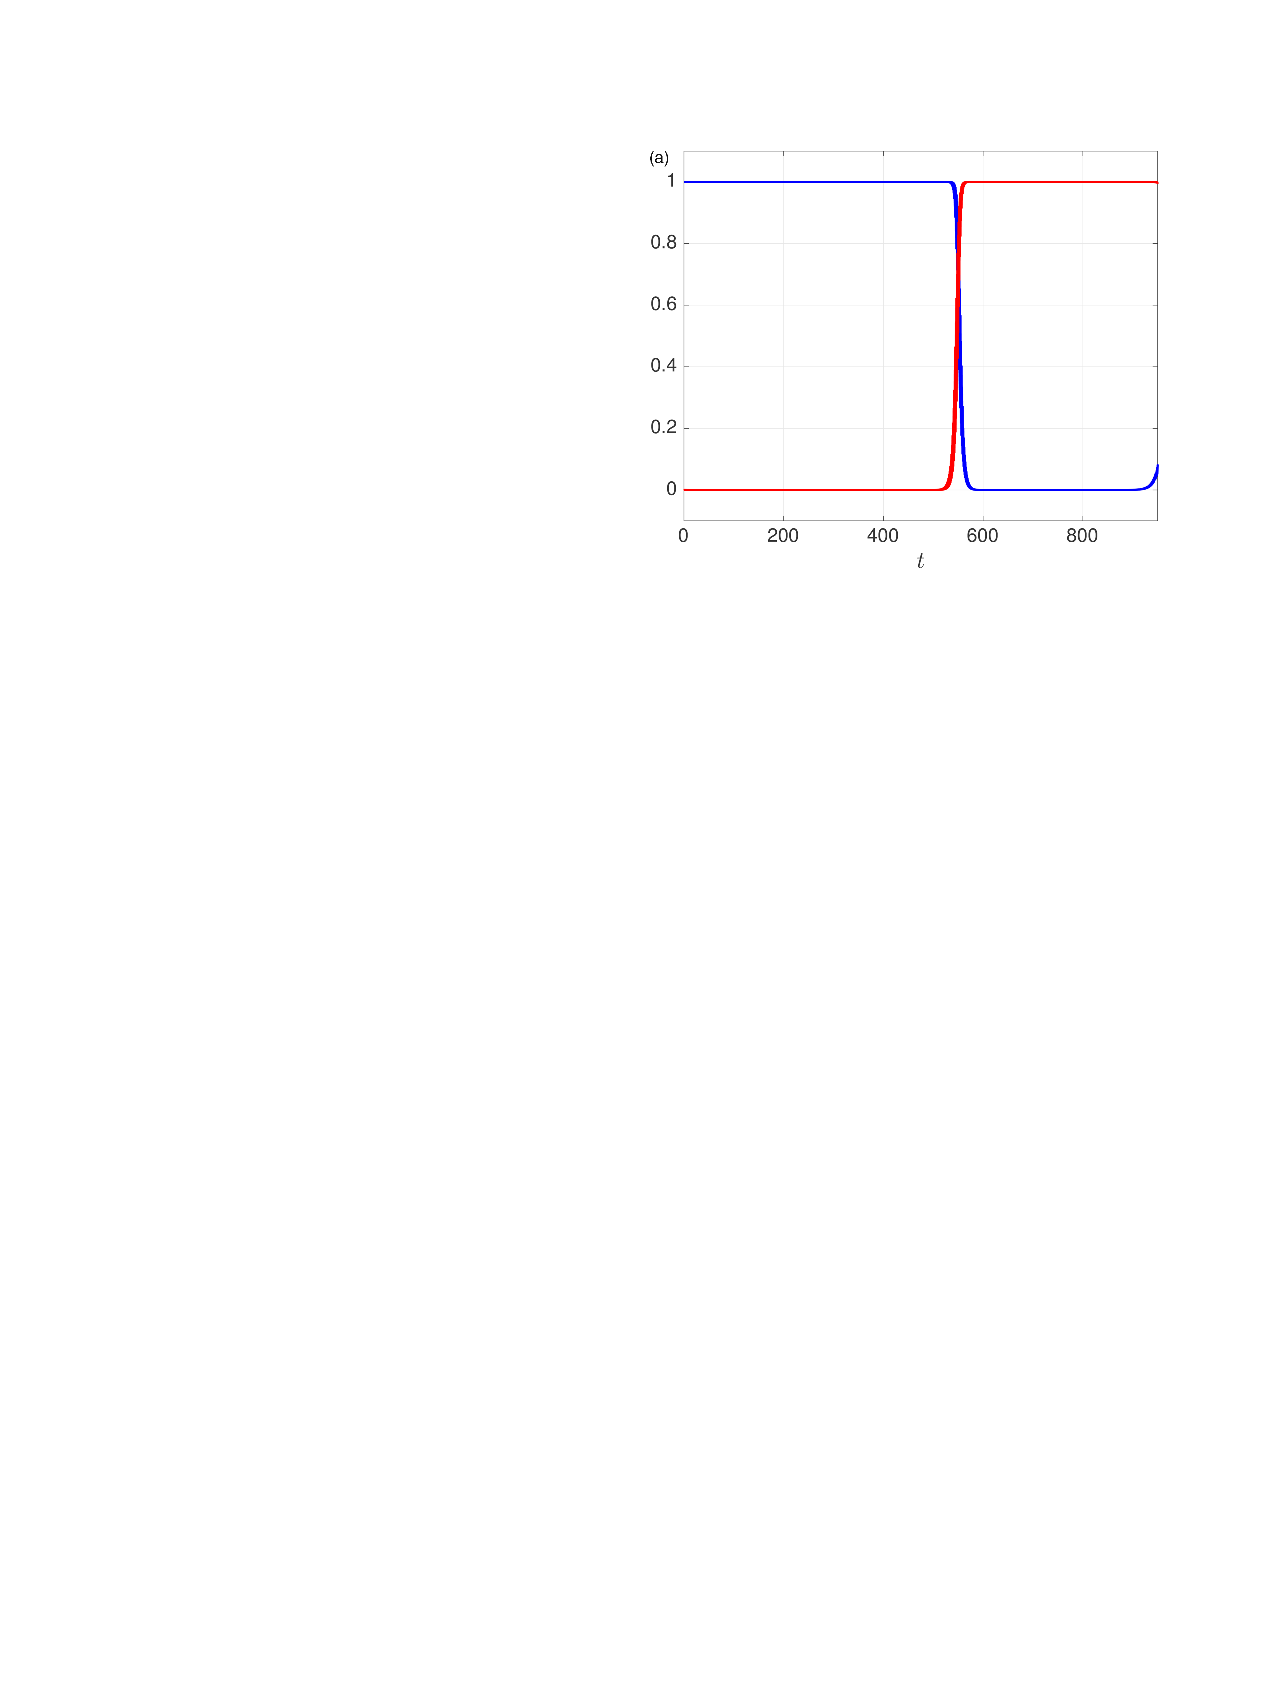
\includegraphics[width=0.5\textwidth]{i/p2.pdf}
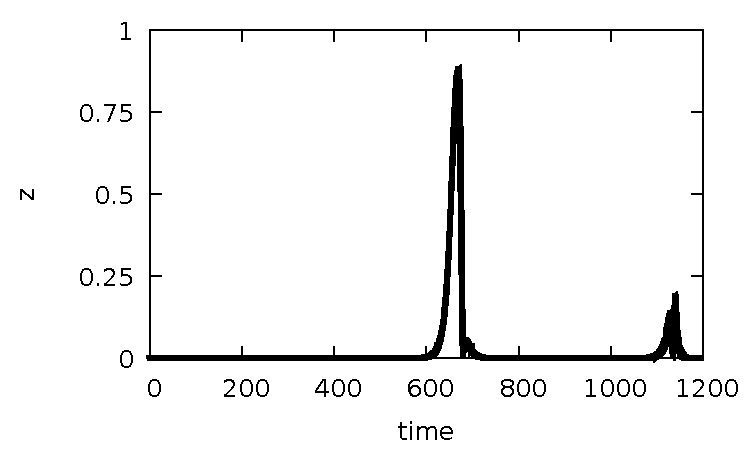
\includegraphics[width=0.5\textwidth]{i/p.pdf}

\eframe
